\documentclass[conference]{IEEEtran}
\usepackage{cite}
\usepackage{graphicx}
\usepackage{caption}
\usepackage{slashbox}

\ifCLASSINFOpdf
  % \usepackage[pdftex]{graphicx}
  % declare the path(s) where your graphic files are
  % \graphicspath{{../pdf/}{../jpeg/}}
  % and their extensions so you won't have to specify these with
  % every instance of \includegraphics
  % \DeclareGraphicsExtensions{.pdf,.jpeg,.png}
\else
  % or other class option (dvipsone, dvipdf, if not using dvips). graphicx
  % will default to the driver specified in the system graphics.cfg if no
  % driver is specified.
  % \usepackage[dvips]{graphicx}
  % declare the path(s) where your graphic files are
  % \graphicspath{{../eps/}}
  % and their extensions so you won't have to specify these with
  % every instance of \includegraphics
  % \DeclareGraphicsExtensions{.eps}
\fi
\usepackage{amsmath}
%\usepackage{algorithmic}

\hyphenation{op-tical net-works semi-conduc-tor}


\begin{document}

\title{Prediction of Heart Disease using Machine Learning Techniques}

\author{
\IEEEauthorblockN{Kevin D'Cruz, Chetan Kumar, Abhishek Manoj Kumar,\\
Madhuri Gawali, Apoorva Shivashankar}
\IEEEauthorblockA{CIS 490 Machine Learning\\
University of Massachusetts\\
Dartmouth, Massachusetts, USA\\
Email: \{kdcruz, ckumar, amanojkumar,\\ mgawali1, ashivashankar\}@umassd.edu}\\   %<------ Line breaks in the current column

}
% make the title area
\maketitle
\begin{abstract}
There is a rapid growth of Machine Learning in the Healthcare domain. Articles and research papers have proven Machine Learning results beneficial, accurate and cost efficient across several domains. The project undertaken was to apply three machine learning models on datasets obtained from the UCI machine learning repository. Three datasets chosen were Cleveland, Statlog and Spect Heart Disease datasets, all related to predicting presence or absence of heart diseases in patients. The models applied on these datasets were logistic regression, decision trees and neural networks. The results were obtained by varying parameters for different models. The goal of the project was to check the model consistency on different datasets and find the best suited algorithm for that particular dataset. Results showed that Cleveland and Statlog datasets had logistic regression and decision tree work best and Neural Networks didn’t give accurate results. Neural Networks worked best for the Spect dataset when compared with logistic regression and decision trees.
\end{abstract}

% no keywords

\IEEEpeerreviewmaketitle



\section{Introduction}
A simple search on Google such as ‘Leading cause of death in the world’ returns Heart Disease topping the list. World Health Organization (WHO) shows Ischemic heart disease and stroke to be the main causes for deaths in the world, where the combined deaths were 15 million in 2015. Also, they remained the leading causes of death globally in the last 15 years [1]. Similarly, the statistics from the 2017 report of the American Heart Association showed Cardiovascular disease (CVD) death count approximately around 800,000 in the United States (US), or one out of every three deaths. Majority of CVD deaths were caused by Coronary heart disease (CHD), followed by stroke and heart failure [2]. Globally, 31\% of deaths were caused from CVD. An estimation carried out relating to the cost of therapy for CVD would be \$1,044 billion by 2030. 1 of 20 deaths in the US are from Strokes. As of 2017, death rates caused by strokes have declined. Stroke has become the leading cause of long-term disability in the US [1].\\

Since the last few years, Machine Learning has been very impactful in the Healthcare industry. Some of it’s application area in the Healthcare domain include Medical Imaging Diagnosis, which focusses on Computer Vision and Deep Learning. Apart from these, a few other application areas in Healthcare include Scaled up Medical Data Collection, Drug discovery and Robotic Surgery [3]. Similarly, scope of machine learning in prediction of diseases has been broadening significantly, and Heart Diseases are one of them. Machine Learning techniques improves accuracy in Cardiovascular risk prediction which helps in avoiding patients who don’t require treatment at an initial stage rather than mistreating them which would put  physical and financial burden on the patients [4].\\

The project carried out by Group 8 was to compare 3 machine models on 3 similar datasets. The 3 datasets used for prediction were: Cleveland, Statlog and Spect Heart Disease Datasets. All the three datasets were related to Heart Diseases. All these datasets were picked from the UCI Machine Learning Repository. These Datasets had Binary Classification which were prediction of presence and absence of heart diseases. The Machine Learning techniques that we used for working on them were: Logistic Regression, Decision trees and Neural Networks. The reason for choosing similar datasets was to check the consistency of these three models or as to how these models performed on datasets having similar attributes and characteristics. The main goal of this project was to determine which model worked the best from the three, based on different evaluation criteria. The models selected were narrowed down from a literature review which is be mentioned in Related Work section.

\section{Related Work}
The models selected for the project goal were based on the review papers as follows: Heart Disease Prediction using Machine Learning and Data Mining Techniques [5]. This paper compared three algorithms based on Decision Tree Classification. They were J48, Logistic Model tree and Random Forest. The J48 algorithm is an extension of the ID3 (Iterative Dichotomiser) model; implemented with Reduced-tree pruning. It had one of the fastest pruning models and produced small and accurate small decision tree rules. A few of the drawbacks of J48 were that the algorithm had a large space complexity as well as large tree sizes. The J48 rules also slowed for noisy and large datasets. The Logistic model carried out cost complexity pruning and used cross-validation for more stable results [5]. The challenge with this algorithm was that it was slower when compared to the other algorithms significantly. The third algorithm mentioned in this paper was the Random Forest Algorithm. This is an ensemble classifier model, and consisted of many decision trees. Random Forest is an improvisation over the Bagging Algorithm. It combines with a random selection of classifiers to construct decision trees with a controlled number of variations [5]. The paper evaluated and concluded by comparing the three algorithms and showed that J48 had a higher sensitivity and accuracy whereas Logistic model tree had higher specificity than J48 and Random Forest. The best model, based on overall performance was J48, considering higher accuracy and least total build time [5].\\

The second relative paper towards the project was: Classification and Prediction of Heart Disease Risk Using Data Mining Techniques of Support Vector Machine and Artificial Neural Networks [6]. This paper used the Cleveland and the Statlog datasets. The goal of this paper was to analyze the prediction variability of two class and multiclass problems. The algorithms used and compared for this were Support Vector Machines and Artificial Neural Networks [6]. SVM is used to classify data, mainly used for two classes and utilizes both kernel and non-kernel functions. SVM had an accuracy of 84.7\% and a precision of 85.06\%. After analysis, the results showed that SVM was a more viable solution than ANN. However, ANN had advantage of performing better in terms of Specificity and Adaptability to extensive training. ANN had an accuracy of 81.8\% and a precision of 83.3\%, slightly lesser than SVM. In terms of Specificity, ANN outperformed SVM [6].\\

\section{Datasets, Methods and Simulation Settings}
\subsection{Datasets}
A brief description of the three datasets used: The Cleveland dataset had 14 attributes (categorical, Integer and Real) and 304 instances. The 'num' attribute is the response variable, used for the prediction. The Statlog Dataset, like the Cleveland, had 14 Attributes (Categorical, Integer and Real) and 270 Instances. Both these datasets were balanced (equal presence and absence outcomes). The spect dataset was different from the first two. It had 23 attributes, with a given training and testing split already. The response variable here was 'Overall\_Diagnosis'. This dataset had features obtained from images, instead of numbers. Also, this dataset was slightly imbalanced, when compared with the first two. 
\subsection{Methods}
The first method or machine learning model performed on the datasets was Logistic Regression. This model is a Statistical method that analyses a dataset having one or more independent variables to determine an outcome [7]. The outcome is measured with a dichotomous variable, which means there could be two possible outcomes (True or False). Logistic Regression is used when finding the best fit model to describe the relationship between the dependent variable and set of independent variables [7].\\

\begin{figure}
	\centering
	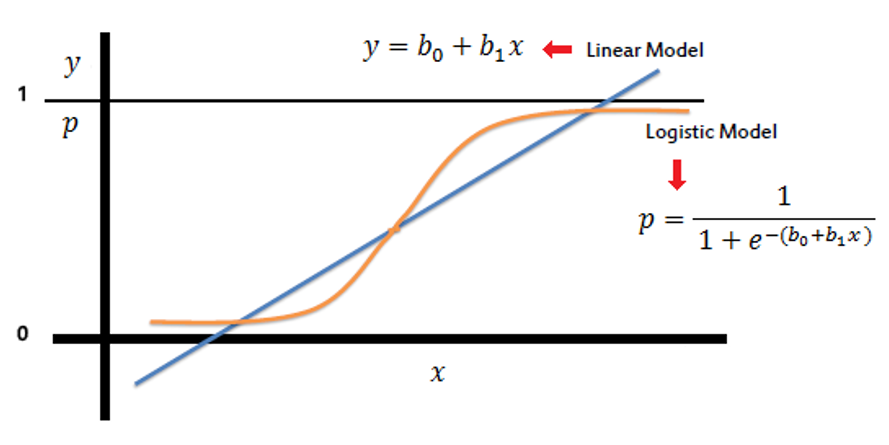
\includegraphics[height=4cm, width=8cm]{images/lr}
	\linebreak
	\captionof{figure}{Logistic Regression}
	\label{fig:logistic-regression-graph}
\end{figure}

The Logistic Regression Figure \ref{fig:logistic-regression-graph} shows the logistic curve (between 0 and 1). The Linear model equation is: $y=b_0 + b_1x$, where $b_0$ is the constant and $b_1$ is the slope which defines the steepness of the curve. The Logistic model equation is in terms of the odd’s ratio. Hence, as seen: $p = 1/ (1+e-( b_0 + b_1x))$ [8].\\

The second model was Decision Trees. They are a type of Supervised Learning method, which works for both categorical and continuous input and output variables. Decision trees are graphic module of Decision Matrix Analysis, and consist of three types of nodes: decision nodes, chance event nodes and terminating nodes [9]. They split the population or sample into two or more homogeneous sets (or sub-populations) based on most significant splitter or differentiator in input variables and if there is a high non-linearity and complex relationship between dependent and independent variables, a tree model will outperform a classical regression method [9]. A decision tree model does significantly better than a linear model and are simpler to interpret than linear regression.\\

Followed by decision trees, we carried out Bagging and Boosting on the datasets. Bagging is a bootstrap model which randomly generates L set of cardinality N from the original set Z with replacement and corrects the optimistic bias of the R-Method [10]. Referred to as Bootstrap Aggregation, Bagging creates Bootstrap samples of a training set using sampling with replacement. Each bootstrap sample is trains a different component of the base classifier and the Classification is done by plurality voting [10]. Regression is carried out by averaging. This technique works for unstable classifiers such as Neural Networks and Decision Trees. Also, Random Forests Algorithm is a Bagging-Variant and is a general class of ensemble building methods using a decision tree as a base classifier.  The main reason for error in learning is due to noise, bias and variance. Noise is error by the target function whereas bias occurs when the algorithm cannot learn the target. Variance comes from the sampling, and how it affects the learning algorithm. These errors are reduced by Bagging and Averaging over bootstrap samples could reduce errors from variance especially considering unstable classifiers [10]. Boosting is a technique which combines multiple base classifiers whose combined performance is significantly better than that of any of the base classifiers. It follows a sequential training of weak learners and each base classifier is trained on weighted data based on the previous classifiers performance [10].\\

The third machine learning model implemented was Neural Networks. An Artificial Neural Network (ANN) is an information processing paradigm; inspired by the way biological nervous systems, such as the brain processes information. It is composed of many highly interconnected processing elements (neurons) working in unison to solve specific problems [11]. Neural Network model was chosen on our datasets is because of it’s adaptive learning ability which learns how to do tasks based on the data given for training or initial experience. Also, self-organization, where an ANN creates its own organization or representation of the information it receives during learning time. ANN also supports Real Time Operation where computations can be carried out in parallel, along with special hardware devices being designed and manufactured taking advantage of this capability [11].\\

We carried out the experiments with 3 modeling techniques for all 3 datasets, but we show the results in detail for each model only once with the dataset which gave us the best results. So we show results for logistic regression and decision trees on Cleveland dataset and neural networks for Spect dataset.

\subsection{Simulations}
The simulation settings or evaluation criteria carried out for logistic regression were as follows data split ratio. The Accuracy and Error rate of the model was calculated based on three different data splits of Training and Testing data which were: (70\% - 30\%), (80\% - 20\%) and (90\% - 10\%). (2) The next evaluation criteria carried out was comparing the Accuracy and the Error in two scenarios; one, considering all the variables and second, considering significant variables. The significant variables obtained by logistic regression are shown in Figure: \ref{fig3}. We consider the first 5 variables which includes ca, thal, sex, exang and trestbps for significant variables. The third evaluation criteria carried out was Cross validation performed on 5 different folds (5, 10, 15, 20 and 25). The last evaluation criteria carried out was generating the ROC Cure for all variables and the significant variables respectively.

\begin{figure}
	\centering
	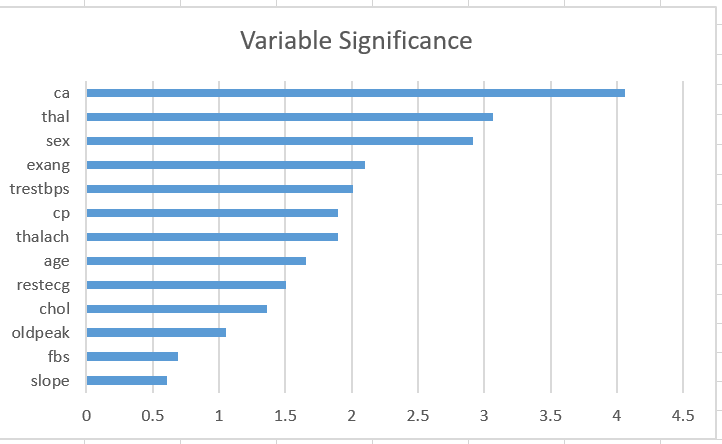
\includegraphics[height=4cm, width=8cm]{images/Fig3}
	\linebreak
	\captionof{figure}{Significant Variable }
	\label{fig3}
\end{figure}

\subsection{Results:}

Considering Logistic Regression on the Cleveland dataset, the accuracy and the error for all the variables obtained are shown in \ref{fig4}. The training accuracy for all the three splits was somewhat, the same (83-84\%). The testing accuracy obtained, was higher (88\%) than the training for the 70-30\% and the 90-10\% split. It was lower than the training accuracy for the 80-20\% split (83\%). For significant variables, the training accuracy obtained was higher for 70-30\% but dropped a percent for the other 2 splits. The testing splits for the significant variables, however, was much lower when compared with all the variables. It dropped down to 77\%. See \ref{fig5}. \\

\begin{figure}
	\centering
	\includegraphics[height=4cm, width=8cm]{images/Fig4}
	\linebreak
	\captionof{figure}{Train vs Test Accuracy for All Variables }
	\label{fig4}
\end{figure}

\begin{figure}
	\centering
	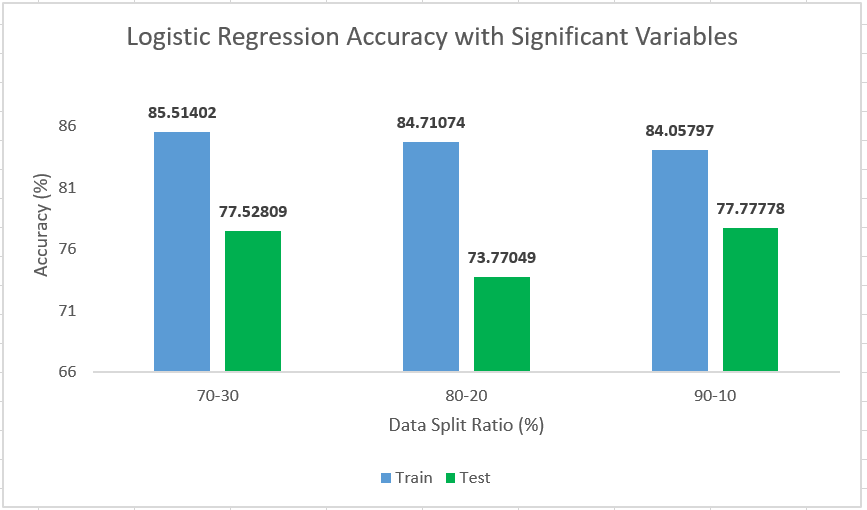
\includegraphics[height=4cm, width=8cm]{images/Fig5}
	\linebreak
	\captionof{figure}{Train vs Test Accuracy for All Variables }
	\label{fig5}
\end{figure}


 Similarly, the Train vs Test Error obtained for the Cleveland Dataset on the three different splits were as follows: The error on the training data was 16\% for the 70-30\% split and around 15\% for 80-20 and 90-10\%. The Test error for three splits were roughly 11\% for 70-30\% and 90-10\% and rose to 16\% for 80-20\%. For Logistic Regression Error of Significant variables, the training error was around 14-15\% and testing error was 22-26\% on different splits. The third Evaluation criteria carried out was Cross Validation. The folds performed were 5, 10, 15, 20 and 25 as seen in Figure:\ref{fig8}.
 
 
 \begin{figure}
 	\centering
 	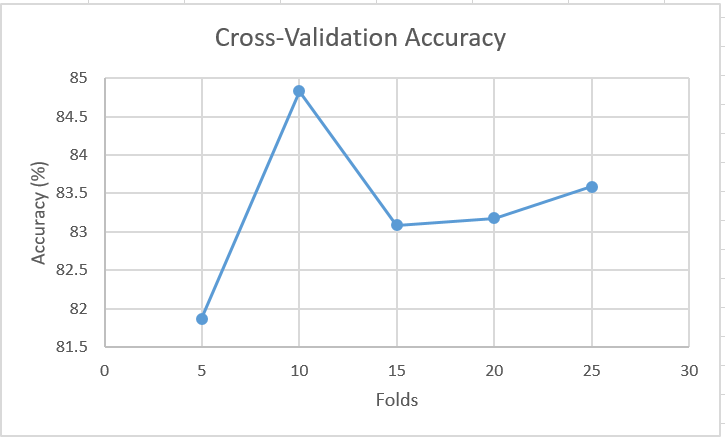
\includegraphics[height=4cm, width=8cm]{images/Fig8}
 	\linebreak
 	\captionof{figure}{Cross-Validation Accuracy on Cleveland Dataset}
 	\label{fig8}
 \end{figure}
 
  
The Line graph shows the accuracy in percentage for the 5 cross-validation folds applied. The lowest was observed at 5 folds with accuracy between 81.5 - 82\%. The highest accuracy obtained was at 10 folds which was 84.9\%, after which there was a decrease and then a slight increase at 25 folds as seen.  
The Final Evaluation was the Area under the curve (AUC), which was the graph of the Specificity (False Positive Rate) against the Sensitivity (True Positive Rate). The AUC for all the variables was 89.13\% whereas for Significant Variables was 86.12\%. The AUC’s obtained are shown in \ref{fig9}
  
\begin{figure}
  	\centering
  	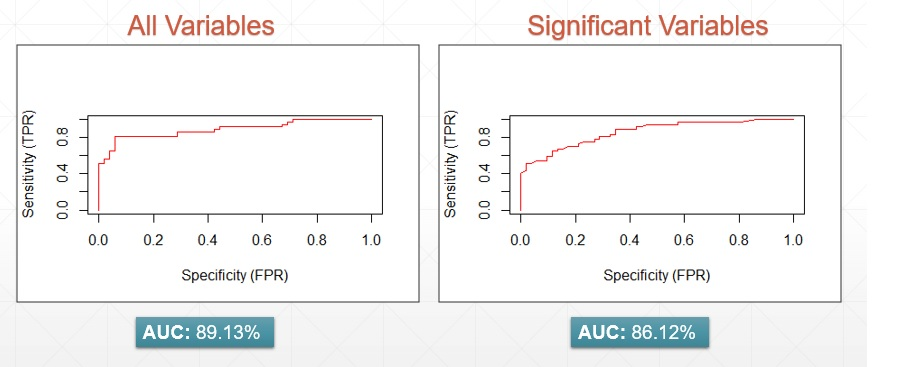
\includegraphics[height=4cm, width=8cm]{images/Fig9}
  	\linebreak
  	\captionof{figure}{AUC of Cleveland Dataset for All and Significant Variables}
  	\label{fig9}
\end{figure}
  
\subsubsection{Decision Tree}
The evaluation criteria for the Decision tree model on the Cleveland Dataset were: Fully Grown Tree, Pruning Tree and Ensemble Learning (Bagging and Boosting). The fully Grown Tree is shown Figure: \ref{fig10}. The Error Percentage for the Cleveland Dataset obtained was 20.22\% 
\begin{figure}
	\centering
	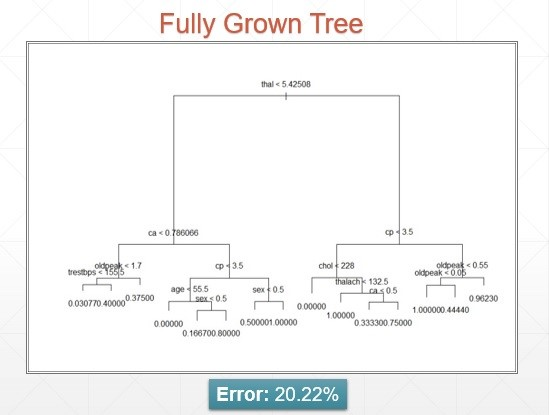
\includegraphics[height=4cm, width=8cm]{images/Fig10}
	\linebreak
	\captionof{figure}{Full Grown Tree: Cleveland Dataset}
	\label{fig10}
	\end{figure}

The Pruning Criteria and the Pruned Tree for the Cleveland Dataset is shown in Fig 11. The Pruning Criteria obtained Best, was 8 and the graph obtained was based on tree size against tree error rate. The graph shows that the best pruning criteria obtained was with a pruned tree having 8 leaf nodes. Similarly, Figure: \ref{fig11} also shows the pruned tree generated once the best pruning criteria was obtained. The Error \% of the Pruned Tree for the Cleveland Dataset was 13.08\%, roughly around 7\% less than the fully grown tree.\\

\begin{figure}
	\centering
	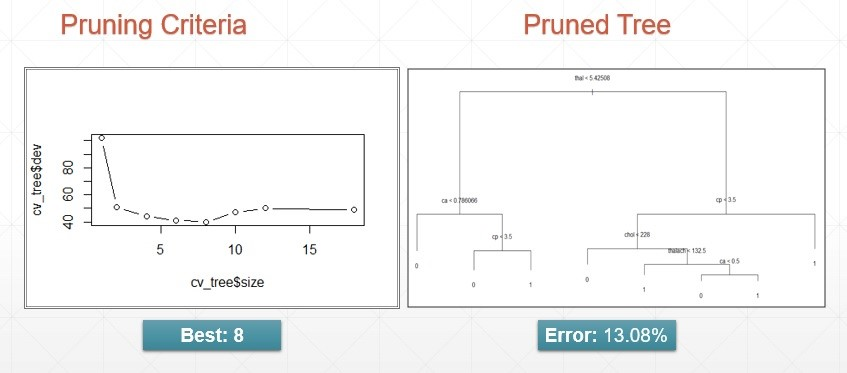
\includegraphics[height=4cm, width=8cm]{images/Fig11}
	\captionof{figure}{Pruning Criteria and Pruned Tree for the Cleveland Dataset}
	\label{fig11}
\end{figure}

The Random Forest Algorithm (Bagging) for a Tree size of 500 is shown in Figure \ref{fig14}. The black line on the plot shows the overall error, the green and red lines show the mean square error for different class labels i.e. 0 and 1. It can be seen that the error is gradually decreasing with increasing number of trees.
\begin{figure}
	\centering
	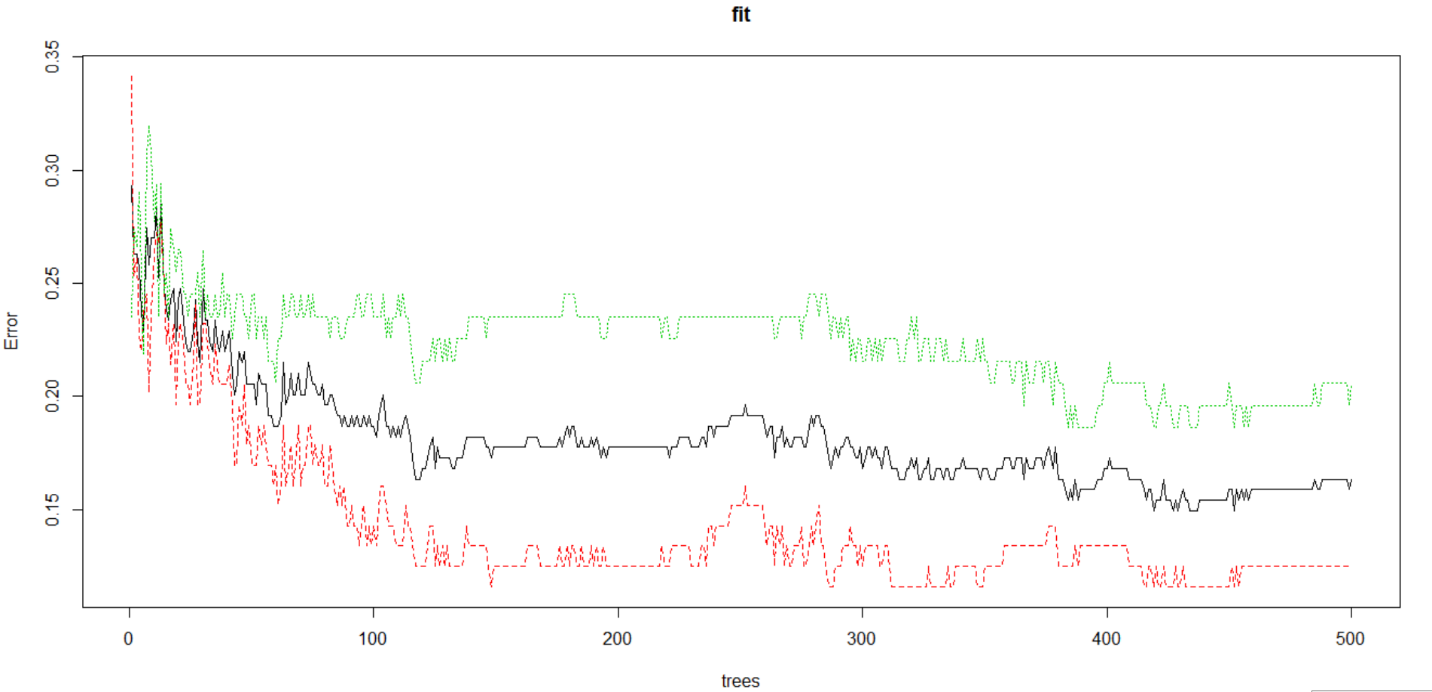
\includegraphics[height=4cm, width=8cm]{images/Fig14}
	\captionof{figure}{Pruning Criteria and Pruned Tree for the Cleveland Dataset}
	\label{fig14}
\end{figure}


For Boosting, the Gradient Boosted Model, is shown in Figure \ref{fig15}. The Performance of Boosting Model on the test set of the Cleveland Dataset along with the table is shown below. The Relative influence of each variable found by gradient boosting model is seen in Figure: \ref{fig16}. It signifies the influence each variable has on the model.

\begin{figure}
	\centering
	\includegraphics[height=4cm, width=8cm]{images/Fig15}
	\captionof{figure}{Performance of Boosting on the test set of Cleveland Dataset}
	\label{fig15}
\end{figure}

\begin{figure}
	\centering
	\includegraphics[height=4cm, width=8cm]{images/Fig16}
	\captionof{figure}{Relative Influence}
	\label{fig16}
\end{figure}



\subsubsection{Neural Network}
We found interesting results on the third model, neural networks. For the first two datasets, Cleveland and statlog, the predictions were only for one class with test accuracy of 58.42 and 50.23\% respectively. We observed that neural networks didn’t work well for Cleveland and statlog datasets. For the 3rd dataset, SPECT, we found that neural networks gave good results and we describe these results in detail. 
The various evaluation criteria we used for neural networks were, split ratio, where we used different splits of train and test data to find deviation in accuracy and errors, if any. The second criteria was to vary the number of hidden layers, followed by the type of algorithm we used to train the neural network which includes backpropagation and resilient backpropagation. We also varied the learning rate which is used to update the inter-neuronal synaptic weights during each training iteration. The snapshot of the neural network on Spect dataset is shown in Figure \ref{fig17}.

\begin{figure}
	\centering
	\includegraphics[height=4cm, width=8cm]{images/Fig17}
	\captionof{figure}{: Snapshot of the neural network with 3 hidden layers.}
	\label{fig17}
\end{figure}

The results we obtained are summarized below, we obtained similar accuracies for different data splits and on the train set, accuracy ranged from 93 to 94 percent with the highest training accuracy of 94.46\% obtained for 90 percent train data and the highest test accuracy of 81.13\% for 20 percent test data.  Figure: \ref{fig18} shows these results,\\

\begin{figure}
	\centering
	\includegraphics[height=4cm, width=8cm]{images/Fig18}
	\captionof{figure}{Neural Network on Different Data Splits}
	\label{fig18}
\end{figure}

\begin{figure}[h!]
	\centering
	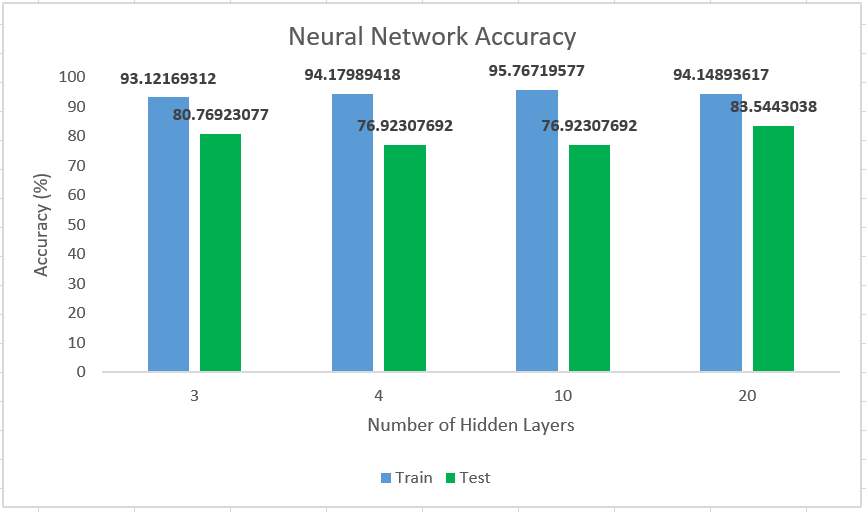
\includegraphics[height=4cm, width=8cm]{images/Fig19}
	\captionof{figure}{Neural Network Accuracy with Different Number of Hidden Layers}
	\label{fig19}
\end{figure}

The second criteria we tested was varying the number of hidden layers and the results are seen in Figure: \ref{fig19}. The accuracy doesn’t vary by a lot, but some slight changes are observed. The highest train accuracy was 95.76 with 10 hidden layers and the highest test accuracy was 83.54 with 20 hidden layers. This test was performed by using 70:30 split ratio for train and test data and it was kept constant while varying the number of hidden layers. 

\section{Conclusion}
Finally, we show a summary of the best test results of different datasets on the 3 models. And can be seen in table. \\

\begin{tabular}{|l||*{3}{c|}}\hline
	\backslashbox{Methods}{Datasets}
	&\makebox[3em]{Cleveland}&\makebox[3em]{Statlog}&\makebox[3em]{Spect}
	\\\hline\hline
	Logistic Regression &88.88&85.18&65.24\\\hline
	Decision Tree &87.46&88.65&66.31\\\hline
	Neural Network &58.42&50.23&83.54\\\hline
\end{tabular}

\bigskip


The main goal of this project as described earlier, was to determine the model that worked best for one dataset, based on different evaluation criteria. Hence, from the results obtained, we could conclude that for the Cleveland and Statlog datasets, the Logistic Regression and Decision trees worked the best. The reason for this was that these two datasets were very similar and had similar attributes, including the response variable (num). Logistic Regression and Decision trees worked best since this dataset was based on Binary Classification and both the datasets were quite balanced. 
For the third dataset, SPECT, the best model from the three was Neural Networks. The reason for this was that this dataset consisted of features. The Neural Networks model performed significantly well compared to the other two models. Both Logistic Regression and Decision Trees didn’t work, since the data included was feature data and not demographic data. Also, this dataset was quite imbalanced when compared with the other two datasets.

\section*{Contribution}
The contributions are as follows:
Kevin D’cruz worked on background research, research on data selection and implementation and project report.
Chetan Kumar worked on tools, libraries and packages, implementation and project report.
Abhishek Manoj Kumar worked on implementation, research on methodology and project report.
Madhuri gawali worked on research on method selection and project report.
Apoorva shivashankar worked n literature review and project report. 
All the members had almost the same contribution in the project.



\begin{figure}[h!]
	
	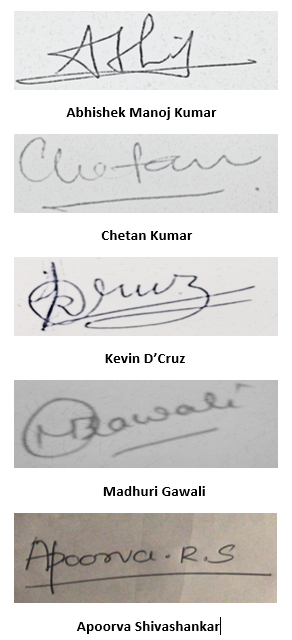
\includegraphics[height=10cm, width=4cm]{images/signature}
	\label{fig20}
\end{figure}



\section*{References}
[1]http://www.who.int/mediacentre/factsheets/fs310/en/ 

[2]http://www.acc.org/latest-in-cardiology/ten-points-to-remember/2017/02/09/14/58/heart-disease-and-stroke-statistics-2017 

[3]https://www.techemergence.com/machine-learning-healthcare-applications/

[4]http://journals.plos.org/plosone/article/file?id=10.1371/journal\\.pone.017494we 4\&type=printable 

[5]http://csjournals.com/IJCSC/PDF7-1/18.\%20Tejpal.pdf

[6]http://ieeexplore.ieee.org/document/7724835/

[7]http://dsd.future-lab.cn/members/2015nlp/Machine\_Learning\\.pdf

[8]http://www.saedsayad.com/logistic\_regression.htm

[9]Lecture Notes

[10]https://www.cs.rit.edu/~rlaz/prec20092/slides/Bagging\_and\\\_Boosting.pdf

[11]https://www.doc.ic.ac.uk/~nd/surprise\_96/journal/vol4/cs11/\\report.html
% trigger a \newpage just before the given reference

% number - used to balance the columns on the last page
% adjust value as needed - may need to be readjusted if
% the document is modified later
%\IEEEtriggeratref{8}
% The "triggered" command can be changed if desired:
%\IEEEtriggercmd{\enlargethispage{-5in}}

% references section

% can use a bibliography generated by BibTeX as a .bbl file
% BibTeX documentation can be easily obtained at:
% http://mirror.ctan.org/biblio/bibtex/contrib/doc/
% The IEEEtran BibTeX style support page is at:
% http://www.michaelshell.org/tex/ieeetran/bibtex/
%\bibliographystyle{IEEEtran}
% argument is your BibTeX string definitions and bibliography database(s)
%\bibliography{IEEEabrv,../bib/paper}
%
% <OR> manually copy in the resultant .bbl file
% set second argument of \begin to the number of references
% (used to reserve space for the reference number labels box)
%\bibliographystyle{IEEEtran}
%\bibliography{IEEEfull,mybib}







% that's all folks
\end{document}


